\documentclass[12pt, letterpaper, titlepage]{article}
\usepackage[utf8]{inputenc}

\usepackage{geometry}
\usepackage{color,graphicx,overpic,colortbl} 
\usepackage{fancyhdr}
\usepackage{amsmath,amsthm,amsfonts,amssymb}
\usepackage{mathtools}
\usepackage{hyperref}
\usepackage{multicol}
\usepackage{array}
\usepackage{float}
\usepackage{blindtext}
\usepackage{longtable}
\usepackage{scrextend}
\usepackage[font=small,labelfont=bf]{caption}
\usepackage{calc}
\usepackage{titlesec}
\usepackage{listings}
\usepackage[normalem]{ulem}
\usepackage{tabularx}
\usepackage{mathrsfs}
\usepackage{bookmark}
\usepackage{setspace}
\usepackage{ragged2e}
\usepackage{ltablex}
\usepackage{xurl}
\usepackage{tikz}
\usepackage{pgfplots}
\usepackage{xparse}

\usepackage{xcolor}

\lstdefinestyle{style}{
    frame=L,
    xleftmargin=\parindent,
    belowcaptionskip=1\baselineskip,
    basicstyle=\footnotesize\ttfamily,
    keywordstyle=\bfseries\color{teal!40!black},
    commentstyle=\itshape\color{purple!40!black},
    identifierstyle=\color{blue},
    stringstyle=\color{cyan},
    breakatwhitespace=false,         
    breaklines=true,                 
    captionpos=b,                    
    keepspaces=true,                                 
    showspaces=false,                
    showstringspaces=false,
    showtabs=false,                  
    tabsize=2,
}

\pgfplotsset{width=8cm,compat=1.15}\usepgfplotslibrary{patchplots}
\mathtoolsset{showonlyrefs}  
\allowdisplaybreaks

\definecolor{mycolor}{rgb}{0, 0, 0}

\geometry{top=2.54cm, left=2.54cm, right=2.54cm, bottom=2.54cm}
\setlength{\headheight}{20pt}
\setlength{\parskip}{0.3cm}
\setlength{\parindent}{1cm}

\pagestyle{fancy}
\fancyhf{}
\rhead{Lora Ma - 1570935}
\lhead{\textit{ECE 322 Lab 3}}
\rfoot{Page \thepage}

\begin{document} 
\singlespacing

\section{Introduction}
The purpose of this lab is to become familiar with integration white-box testing. The goal of this lab was to give us experience with using Python and Python unittest unittest.mock for integration testing.

Integration testing serves as a logical extensions of unit testing. There are two general approaches to integration testing -- non-incremental testing (Big Bang) and incremental testing (Top down/Bottom up). In non-incremental testing, each module is tested individually and then the whole system is tested as a whole. In integration testing, we combine the next module to be tested with the set of previously tested modules before running tests. This can generally done in either a bottom up or top down method. A bottom up method involves testing the lowest level modules in isolation and then incrementally adding higher and higher module levels. A top down method involves testing the highest level modules in isolation and then incrementally adding lower modules.

Integration testing usually involves using various stubs and drivers. Stubs, in integration testing, is used as a stand in for lower level modules that are not currently under test. A stub returns a dummy value or makes an assertion so that the test case can ensure it was called. Drivers are a piece of testing code which makes it possible to call a submodule of an application independently.

In this lab, we will be focusing on non-incremental testing

\section{Non-incremental testing - Big Bang testing}
During the non-incremental testing portion of this lab, we made unit tests for module A-F along with test cases for the system as a whole. For each module, we mocked any dependencies on other modules. You can find the tests in the directory src/tests. In the test case table on the next page, the red highlighted entries are failed test cases.

\begin{table}[H]
    \centering
    \caption{Test results for non-incremental testing}
    \label{tab:my-table}
    \begin{tabular}{|l|l|l|l|}
    \hline
    \textbf{Test \#} & \textbf{Module} & \textbf{Test name}            & \textbf{Passed?} \\ \hline
    1                & A               & test\_allCommands             & Pass             \\ \hline
    2                & A               & test\_allCommandsIndexError   & Pass             \\ \hline
    3                & A               & test\_allCommandsNoFile       & Pass             \\ \hline
    4                & A               & test\_dataGetter              & Pass             \\ \hline
    5                & A               & test\_dataSetter              & Pass             \\ \hline
    6                & A               & test\_help                    & Pass             \\ \hline
    7                & A               & test\_noCommand               & Pass             \\ \hline
    8                & A               & test\_parseAddWithData        & Pass             \\ \hline
    9                & A               & test\_parseAddWithNoData      & Pass             \\ \hline
    10               & A               & test\_parseDeleteWithValue    & Pass             \\ \hline
    11               & A               & test\_parseDeleteWithoutValue & Pass             \\ \hline
    12               & A               & test\_parseLoadData           & Pass             \\ \hline
    13               & A               & test\_parseLoadNoData         & Pass             \\ \hline
    14               & A               & test\_parseUpdateWithData     & Pass             \\ \hline
    15               & A               & test\_parseUpdateWithNoData   & Pass             \\ \hline
    16               & A               & test\_runExit                 & Pass             \\ \hline
    17               & A               & test\_runSortWithData         & Pass             \\ \hline
    18               & A               & test\_runSortWithNoData       & Pass             \\ \hline
    19               & A               & test\_unknownCmd              & Pass             \\ \hline
    20               & B               & test\_FGetter                 & Pass             \\ \hline
    21               & B               & test\_FSetter                 & Pass             \\ \hline
    22               & B               & test\_IOError                 & Pass             \\ \hline
    \rowcolor[HTML]{FF7F7F} 
    23               & B               & test\_fileNotFoundError       & Fail             \\ \hline
    24               & B               & test\_loadFile                & Pass             \\ \hline
    25               & C               & test\_FGetter                 & Pass             \\ \hline
    26               & C               & test\_FSetter                 & Pass             \\ \hline
    27               & C               & test\_sortData                & Pass             \\ \hline
    28               & D               & test\_FGetter                 & Pass             \\ \hline
    29               & D               & test\_FSetter                 & Pass             \\ \hline
    30               & D               & test\_GGetter                 & Pass             \\ \hline
    31               & D               & test\_GSetter                 & Pass             \\ \hline
    32               & D               & test\_deleteData              & Pass             \\ \hline
    33               & D               & test\_insertData              & Pass             \\ \hline
    \rowcolor[HTML]{FF7F7F} 
    34               & D               & test\_updateData              & Fail             \\ \hline
    35               & E               & test\_exit                    & Pass             \\ \hline
    36               & F               & test\_displayData             & Pass             \\ \hline
    37               & G               & test\_updateData              & Pass             \\ \hline
    38               & G               & test\_updateDataFileNotFound  & Pass             \\ \hline
    \end{tabular}
    \end{table}
\newpage
Additionally, a coverage report is provided below: \\
\begin{center}
    \captionof{figure}{Coverage results for non-incremental testing}
    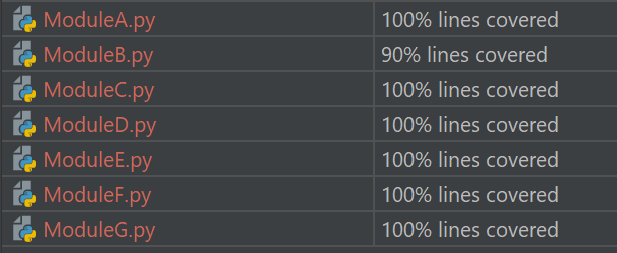
\includegraphics[scale=1.2]{coverageTable.png} 
\end{center}

Out of the 38 tests, only 2 tests (test 23 and test 34) failed. We had 100\% code coverage on all modules except for ModuleB where lines 22 to 26 can not be reached at all. We will explain the failures of the two tests in the following section

\section{Failures}
\subsection{Test 23}
Test 23, named \lstinline{test_fileNotFoundError}, in module B failed. We tried to trigger a \lstinline{FileNotFoundError}, but as mentioned earlier, that section of code is impossible to reach since an error would be caught by the earlier IOError exception as shown below:
\begin{lstlisting}[language=Python, style=style]
    except IOError as e:
        print("Could not read file:{0.filename}".format(e))
    except FileNotFoundError:
        msg = "FileNotFoundError"
        print (msg)
\end{lstlisting}

As you can see, the FileNotFoundError can not be reached. In order to reach this section of code, we need to switch the IOERROR and FileNotFoundError statements like the following:

\begin{lstlisting}[language=Python, style=style]
    except FileNotFoundError:
        msg = "FileNotFoundError"
        print(msg)
    except IOError as e:
        print("Could not read file:{0.filename}".format(e))
\end{lstlisting}

\subsection{Test 34}
Test 34, name \lstinline{test_updateData}, in module D failed. In the test, we used the following data where we were trying to update data at index 2.
\begin{multicols}{2}
    \begin{lstlisting}[language=Python, style=style]
        data = [
            ('A', '1'),
            ('B', '2'),
            ('C', '3'),
            ('D', '4'),
        ]
    \end{lstlisting}

    \begin{lstlisting}[language=Python, style=style]
        expected = [
            ('A', '1'),
            ('B', '2'),
            ('Z', '22'),
            ('D', '4'),
        ]
    \end{lstlisting}
\end{multicols}
This test failed however due to the following line in updateData in ModuleD where when index used, it is incremented by one which produces unexpected results. It does not update the index passed in and instead updates the index above it.
\begin{lstlisting}[language=Python, style=style]
    data[index+1]=Entry(name, number)
\end{lstlisting}
To fix this, we simply remove the +1 in the code like the following:
\begin{lstlisting}[language=Python, style=style]
    data[index]=Entry(name, number)
\end{lstlisting}

\section{Discussion}
Through non-incremental testing, we were able to effectively test the program. We were able to find several errors in our program. This type of testing is good at making sure individual modules are tested and that the modules are also working well together. This type of testing can seem impractical for large projects since it requires a lot of effort to write tests for each module and sometimes there were tests that tested very similar functionality. Creating mocks of modules does seem to be an effective way to mock the functionality of modules to isolate the testing of the module.

\section{Conclusion}
The purpose of this lab was to become familiar with integration white-box testing. The goal of this lab was to teach us to use Python and Python unittest unittest.mock for integration testing. Integration testing is a form of unit testing. We used non-incremental testing also known as big bang testing where every module is tested individually and then the system is tested as a whole. Usually integration testing involves using stubs and drivers to isolate modules to be tested individually.

In this lab, we were able to test modules A-F using non-incremental testing and wrote tests for each module as well as testing the system as a whole. We were able to find 2 failures in the program and explained possible reasons to how those failures may be fixed. Through this lab, we realized that big bang testing is somewhat effective in testing a program although becomes a lot of work for larger systems.

\end{document}